
%% bare_lsens.tex
%% V1.0
%% 2017/07/12
%% by Michael Shell
%% see http://www.michaelshell.org/
%% for current contact information.
%%
%% This is a skeleton file demonstrating the use of IEEE_lsens.cls for
%% an IEEE Sensors Letters paper.
%%
%% Support sites:
%% -- LaTeX Related --
%% http://www.michaelshell.org/tex/ieeetran/
%% http://www.ctan.org/pkg/ieeetran/
%%
%% -- IEEE/Editor/Submission Related --
%% http://www.ieee-sensors.org/
%% http://www.ieee.org/


%%*************************************************************************
%% Legal Notice:
%% This code is offered as-is without any warranty either expressed or
%% implied; without even the implied warranty of MERCHANTABILITY or
%% FITNESS FOR A PARTICULAR PURPOSE! 
%% User assumes all risk.
%% In no event shall the IEEE or any contributor to this code be liable for
%% any damages or losses, including, but not limited to, incidental,
%% consequential, or any other damages, resulting from the use or misuse
%% of any information contained here.
%%
%% All comments are the opinions of their respective authors and are not
%% necessarily endorsed by the IEEE.
%%
%% This work is distributed under the LaTeX Project Public License (LPPL)
%% ( http://www.latex-project.org/ ) version 1.3, and may be freely used,
%% distributed and modified. A copy of the LPPL, version 1.3, is included
%% in the base LaTeX documentation of all distributions of LaTeX released
%% 2003/12/01 or later.
%% Retain all contribution notices and credits.
%% ** Modified files should be clearly indicated as such, including  **
%% ** renaming them and changing author support contact information. **
%%*************************************************************************


% *** Authors should verify (and, if needed, correct) their LaTeX system  ***
% *** with the testflow diagnostic prior to trusting their LaTeX platform ***
% *** with production work. The IEEE's font choices and paper sizes can   ***
% *** trigger bugs that do not appear when using other class files.       ***
% The testflow support page is at:
% http://www.michaelshell.org/tex/testflow/


% Typically, there isn't any need for class options with IEEE Sensors
% Letters papers. The default, and only, text size is 9pt.
\documentclass{IEEE_lsens}
%
% If IEEE_lsens.cls has not been installed into the LaTeX system files,
% manually specify the path to it like:
% \documentclass{../sty/IEEE_lsens}


% *** Do not adjust lengths that control margins, column widths, etc. ***
% *** Do not use packages that alter fonts (such as pslatex).         ***
% There should be no need to do such things with IEEE_lsens.
% (Unless specifically instructed to do so by the IEEE Sensors Letters
% editors, of course.)


% Some very useful LaTeX packages include:
% (uncomment the ones you want to load)


% *** MISC UTILITY PACKAGES ***
%
%\usepackage{ifpdf}
% Heiko Oberdiek's ifpdf.sty is very useful if you need conditional
% compilation based on whether the output is pdf or dvi.
% usage:
% \ifpdf
%   % pdf code
% \else
%   % dvi code
% \fi
% The latest version of ifpdf.sty can be obtained from:
% http://www.ctan.org/pkg/ifpdf
% Also, note that IEEEtran.cls V1.7 and later provides a builtin
% \ifCLASSINFOpdf conditional that works the same way.
% When switching from latex to pdflatex and vice-versa, the compiler may
% have to be run twice to clear warning/error messages.


% The textcomp package can be loaded to get better \textcopyright and
% \textregistered symbols (as is used in the footer of the title page
% of LSENS papers).
\usepackage{textcomp}






% *** CITATION PACKAGES ***
%
\usepackage[noadjust]{cite}
% cite.sty was written by Donald Arseneau
% V1.6 and later of IEEEtran pre-defines the format of the cite.sty package
%  \cite{} output to follow that of the IEEE. Loading the cite package will
% result in citation numbers being automatically sorted and properly
% "compressed/ranged". e.g., [1], [9], [2], [7], [5], [6] without using
% cite.sty will become [1], [2], [5]--[7], [9] using cite.sty. cite.sty's
%  \cite will automatically add leading space, if needed. Use cite.sty's
% noadjust option (cite.sty V3.8 and later) if you want to turn this off
% such as if a citation ever needs to be enclosed in parenthesis.
% cite.sty is already installed on most LaTeX systems. Be sure and use
% version 5.0 (2009-03-20) and later if using hyperref.sty.
% The latest version can be obtained at:
% http://www.ctan.org/pkg/cite
% The documentation is contained in the cite.sty file itself.






% *** GRAPHICS RELATED PACKAGES ***
%
\ifCLASSINFOpdf
  \usepackage[pdftex]{graphicx}
  % declare the path(s) where your graphic files are
  % \graphicspath{{../pdf/}{../jpeg/}}
  % and their extensions so you won't have to specify these with
  % every instance of \includegraphics
  \DeclareGraphicsExtensions{.pdf,.jpeg,.png}
\else
  % or other class option (dvipsone, dvipdf, if not using dvips). graphicx
  % will default to the driver specified in the system graphics.cfg if no
  % driver is specified.
  \usepackage[dvips]{graphicx}
  % declare the path(s) where your graphic files are
  % \graphicspath{{../eps/}}
  % and their extensions so you won't have to specify these with
  % every instance of \includegraphics
  \DeclareGraphicsExtensions{.eps}
\fi
% graphicx was written by David Carlisle and Sebastian Rahtz. It is
% required if you want graphics, photos, etc. graphicx.sty is already
% installed on most LaTeX systems. The latest version and documentation
% can be obtained at: 
% http://www.ctan.org/pkg/graphicx
% Another good source of documentation is "Using Imported Graphics in
% LaTeX2e" by Keith Reckdahl which can be found at:
% http://www.ctan.org/pkg/epslatex
%
% latex, and pdflatex in dvi mode, support graphics in encapsulated
% postscript (.eps) format. pdflatex in pdf mode supports graphics
% in .pdf, .jpeg, .png and .mps (metapost) formats. Users should ensure
% that all non-photo figures use a vector format (.eps, .pdf, .mps) and
% not a bitmapped formats (.jpeg, .png). The IEEE frowns on bitmapped formats
% for line art (i.e., plots, graphs, etc.) as they result in 
% "jaggedy"/blurry rendering of lines and letters as well as large
% increases in file sizes.
%
% You can find documentation about the pdfTeX application at:
% http://www.tug.org/applications/pdftex





% *** MATH PACKAGES ***

\usepackage[T1]{fontenc} % optional enhanced font encoding
\usepackage{amsmath}
% A popular package from the American Mathematical Society that provides
% many useful and powerful commands for dealing with mathematics.
%
% Note that the amsmath package sets \interdisplaylinepenalty to 10000
% thus preventing page breaks from occurring within multiline equations. Use:
\interdisplaylinepenalty=2500
% after loading amsmath to restore such page breaks as IEEEtran.cls normally
% does. amsmath.sty is already installed on most LaTeX systems. The latest
% version and documentation can be obtained at:
% http://www.ctan.org/pkg/amsmath

\usepackage[cmintegrals]{newtxmath}
% A Times compatible math font is required for IEEE Sensors Letters.
% Michael Sharpe's freely available newtxmath package (version 1.451,
% July 28, 2015 or later) is recommended. The cmintegrals option, which
% IEEE_lsens sets as a default upon loading newtxmath, is/was needed to
% obtain the specific style of integral symbol used by the IEEE Sensors
% Letters. However, as of version 1.5 of the newtxmath package, released
% on 2016/08/12, the correct integral symbol is now invoked by default
% and the cmintegrals option is no longer needed and is silently ignored.
% The latest version and documentation can be obtained at:
% http://www.ctan.org/pkg/newtx
\usepackage{bm}
% support for selective bold math 
% The latest version and documentation can be obtained at:
% http://www.ctan.org/pkg/bm




% *** SPECIALIZED LIST PACKAGES ***
%
%\usepackage{algorithmic}
% algorithmic.sty was written by Peter Williams and Rogerio Brito.
% This package provides an algorithmic environment fo describing algorithms.
% You can use the algorithmic environment in-text or within a figure
% environment to provide for a floating algorithm. Do NOT use the algorithm
% floating environment provided by algorithm.sty (by the same authors) or
% algorithm2e.sty (by Christophe Fiorio) as the IEEE does not use dedicated
% algorithm float types and packages that provide these will not provide
% correct IEEE style captions. The latest version and documentation of
% algorithmic.sty can be obtained at:
% http://www.ctan.org/pkg/algorithms
% Also of interest may be the (relatively newer and more customizable)
% algorithmicx.sty package by Szasz Janos:
% http://www.ctan.org/pkg/algorithmicx




% *** ALIGNMENT PACKAGES ***
%
\usepackage{array}
% Frank Mittelbach's and David Carlisle's array.sty patches and improves
% the standard LaTeX2e array and tabular environments to provide better
% appearance and additional user controls. As the default LaTeX2e table
% generation code is lacking to the point of almost being broken with
% respect to the quality of the end results, all users are strongly
% advised to use an enhanced (at the very least that provided by array.sty)
% set of table tools. array.sty is already installed on most systems. The
% latest version and documentation can be obtained at:
% http://www.ctan.org/pkg/array


% IEEEtran contains the IEEEeqnarray family of commands that can be used to
% generate multiline equations as well as matrices, tables, etc., of high
% quality.




% *** SUBFIGURE PACKAGES ***
\usepackage[caption=false,font=footnotesize,labelfont=sf,textfont=sf]{subfig}
% subfig.sty, written by Steven Douglas Cochran, is the modern replacement
% for subfigure.sty, the latter of which is no longer maintained and is
% incompatible with some LaTeX packages including fixltx2e. However,
% subfig.sty requires and automatically loads Axel Sommerfeldt's caption.sty
% which will override IEEEtran.cls' handling of captions and this will result
% in non-IEEE style figure/table captions. To prevent this problem, be sure
% and invoke subfig.sty's "caption=false" package option (available since
% subfig.sty version 1.3, 2005/06/28) as this is will preserve IEEE_lsens.cls
% handling of captions.
%
% The latest version and documentation of subfig.sty can be obtained at:
% http://www.ctan.org/pkg/subfig




% *** PDF, URL AND HYPERLINK PACKAGES ***
%
\usepackage{url}
% url.sty was written by Donald Arseneau. It provides better support for
% handling and breaking URLs. url.sty is already installed on most LaTeX
% systems. The latest version and documentation can be obtained at:
% http://www.ctan.org/pkg/url
% Basic use: \url{my_url_here}.
%
%
% NOTE: PDF hyperlink and bookmark features are not required in IEEE
%       papers and their use requires extra complexity and work.
\newcommand\MYhyperrefoptions{hypertexnames=true, bookmarks=true,
bookmarksnumbered=true, pdfpagemode={UseOutlines}, plainpages=false,
pdfpagelabels=true, colorlinks=true, linkcolor={black},
citecolor={black}, urlcolor={black}}
\ifCLASSINFOpdf
% \usepackage[\MYhyperrefoptions,breaklinks=true,pdftex]{hyperref}
\else
%  \usepackage[\MYhyperrefoptions,dvips]{hyperref}
%  \usepackage{breakurl}
\fi
%
% We will provide for these commands even if hyperref is not loaded to
% allow hyperref to be unloaded without have to delete any apprearances
% of these commands in the document.
\providecommand{\hypersetup}[1]{\relax}
\providecommand{\texorpdfstring}[2]{#1}
%
% We use \hypersetup instead of the package options for the
% PDF strings because there is a problem with using underscores
% with the package option approach. Also, the info that needs
% to be changed is all here. 
% *** IF USING HYPERREF BE SURE AND CHANGE THE EXAMPLE PDF ***
% *** TITLE/SUBJECT/AUTHOR/KEYWORDS INFO BELOW!!
%
\hypersetup{pdftitle={Bare Demo of IEEE\_lsens.cls for IEEE Sensors Letters},%<!CHANGE!
pdfsubject={Typesetting},%<!CHANGE!
pdfauthor={Michael D. Shell},%<!CHANGE!
pdfkeywords={Class, IEEE, IEEE\_lsens, IEEE Sensors Letters, LaTeX, Typesetting, TeX}}%<^!CHANGE!}
%
% One significant drawback of using hyperref under DVI output is that the
% LaTeX compiler cannot break URLs across lines or pages as can be done
% under pdfLaTeX's PDF output via the hyperref pdftex driver. This is
% probably the single most important capability distinction between the
% DVI and PDF output. Perhaps surprisingly, all the other PDF features
% (PDF bookmarks, thumbnails, etc.) can be preserved in
% .tex->.dvi->.ps->.pdf workflow if the respective packages/scripts are
% loaded/invoked with the correct driver options (dvips, etc.). 
% As most IEEE papers use URLs sparingly (mainly in the references), this
% may not be as big an issue as with other publications.
%
% That said, Vilar Camara Neto created his breakurl.sty package which
% permits hyperref to easily break URLs even in dvi mode.
% Note that breakurl, unlike most other packages, must be loaded
% AFTER hyperref. The latest version of breakurl and its documentation can
% be obtained at:
% http://www.ctan.org/pkg/breakurl
% breakurl.sty is not for use under pdflatex pdf mode.
%
% The advanced features offer by hyperref.sty are not required for IEEE
% submission, so users should weigh these features against the added
% complexity of use.
% The package options above demonstrate how to enable PDF bookmarks
% (a type of table of contents viewable in Acrobat Reader) as well as
% PDF document information (title, subject, author and keywords) that is
% viewable in Acrobat reader's Document_Properties menu. PDF document
% information is also used extensively to automate the cataloging of PDF
% documents. The above set of options ensures that hyperlinks will not be
% colored in the text and thus will not be visible in the printed page,
% but will be active on "mouse over". USING COLORS OR OTHER HIGHLIGHTING
% OF HYPERLINKS CAN RESULT IN DOCUMENT REJECTION BY THE IEEE, especially if
% these appear on the "printed" page. IF IN DOUBT, ASK THE RELEVANT
% SUBMISSION EDITOR. You may need to change/add the option for
% hypertexnames=false if you used duplicate equation numbers, etc., but
% this should not be needed in normal IEEE work.
% The latest version of hyperref and its documentation can be obtained at:
% http://www.ctan.org/pkg/hyperref



% correct bad hyphenation here
\hyphenation{op-tical net-works semi-conduc-tor}


\begin{document}


% The paper headers
\markboth{Vol.~1, No.~3, July~2017}{0000000}


% article subject line 
\IEEELSENSarticlesubject{Sensor Applications}


% paper title
% Titles are generally capitalized except for words such as a, an, and, as,
% at, but, by, for, in, nor, of, on, or, the, to and up, which are usually
% not capitalized unless they are the first or last word of the title.
% Linebreaks \\ can be used within to get better formatting as desired.
% Do not put math or special symbols in the title.
%
\title{Multi-view Scene Image Inpainting Based on Conditional Generative Adversarial Networks}


% author names and IEEE memberships
% note positions of commas and nonbreaking spaces ( ~ ) LaTeX will not break
% a structure at a ~ so this keeps an author's name from being broken across
% two lines.
% use \thanks{} to gain access to the first footnote area
% a separate \thanks must be used for each paragraph as LaTeX2e's \thanks
% was not built to handle multiple paragraphs
%
\author{\IEEEauthorblockN{Michael~Shell\IEEEauthorrefmark{1}\IEEEauthorieeemembermark{1}, John~Doe\IEEEauthorrefmark{2},
and~Jane~Doe\IEEEauthorrefmark{2}\IEEEauthorieeemembermark{2}}% <-this % stops a space
\IEEEauthorblockA{\IEEEauthorrefmark{1}Department of Electrical and Computer Engineering,
Georgia Institute of Technology, Atlanta, GA, 30332, USA\\
\IEEEauthorrefmark{2}Indian Institute of Engineering Science and Technology, Shibpur, Howrah 711103, India\\
\IEEEauthorieeemembermark{1}Member, IEEE\\
\IEEEauthorieeemembermark{2}Senior Member, IEEE}%
% LSENS authors should provide a real e-mail address here.
\thanks{Corresponding author: M. Shell (e-mail: nospam@nospam.org).\protect\\
(For the real e-mail address, see http://www.michaelshell.org/contact.html).}% <-this % stops a space
\thanks{Associate Editor: Alan Smithee.}%
\thanks{Digital Object Identifier 10.1109/LSENS.2017.0000000}}
%
% note the % following lines that end in } - 
% these prevent an unwanted space from occurring between the objects.
% i.e., if you had this:
% 
% \author{....lastname \thanks{...} \thanks{...} }
%                     ^------------^------------^----Do not want these spaces!
%
% a space would be appended to the last name and could cause every name on that
% line to be shifted left slightly. This is one of those "LaTeX things". For
% instance, "\textbf{A} \textbf{B}" will typeset as "A B" not "AB". To get
% "AB" then you have to do: "\textbf{A}\textbf{B}"
% \thanks is no different in this regard, so shield the last } of each \thanks
% that ends a line with a % and do not let a space in before the next \thanks.
% For what it is worth, this is a minor point as most people would not even
% notice if the said evil space somehow managed to creep in.


% Manuscript received line
\IEEELSENSmanuscriptreceived{Manuscript received June 7, 2017;
revised June 21, 2017; accepted July 6, 2017.
Date of publication July 12, 2017; date of current version July 12, 2017.}


% for Sensors Letters papers, we must declare the abstract and index terms
% PRIOR to the title within the \IEEEtitleabstractindextext IEEEtran
% command as these need to go into the title area created by \maketitle.
% As a general rule, do not put math, special symbols or citations
% in the abstract or keywords.
\IEEEtitleabstractindextext{%
\begin{abstract}
Multi-views systems have been widely used in robots, ADAS(Advanced Driver Assistance Systems), monitor systems and so on, using multi-views, the machine can better perceive the surrounding scenes. The exposed lens and the camera are easily contaminated by the outside, resulting in abnormal images. Image inpainting technology can utilize the prior information of the image structure, texture and other information provided by the surrounding pixels of the abnormal area to recover the damaged image, which can reduce the loss of visual information, providing as much information as possible for the machine's decisions. In order to achieve the above purposes, considering the characteristics of multi-vision system, a novel image inpainting method is proposed. The basic idea is that using conditional generative adversarial networks(CGAN) to amend defect images, in which the priori condition is the synchronization frame from other cameras in different viewpoints. The generator in the CGAN is a autoencoder which has skip connected from encoder to decoder. We also integrate spatial transform networks, group convolution and channel switching technology in our network structure to better fusion the multi-views information. Experimental results show the advantage of our method.
\end{abstract}

\begin{IEEEkeywords}
Image inpainting, generative adversarial networks, convolutional neural network, deep learning.
\end{IEEEkeywords}}


% If you want to put a publisher's ID mark on the page you can do it like
% this:
\IEEEpubid{1949-307X \copyright\ 2017 IEEE. Personal use is permitted, but republication/redistribution requires IEEE permission.\\
See \url{http://www.ieee.org/publications\_standards/publications/rights/index.html} for more information.}
% Remember, if you use this you must call \IEEEpubidadjcol in the second
% column for its text to clear the IEEEpubid mark.


% make the title area
\maketitle

\section{Introduction}

Image inpainting means to restore the defective image according to the image texture, structure and other information. It has been broad applied in many field, such as defect images restoration  \cite{Efros1999::Texture,Lu2010::Novel}, video communication error repairing \cite{Rane2002::Wavelet,Rane2003:IToIP:Structure} and photo editing \cite{Bertalmio2000::Image,Shih2005::Digital}. With the development of image and video processing technology, visual information has played a key role in the field  of automation. Due to the limited information available from monocular cameras, the multi-views system is widely used. Fig \ref{fig:VehicleWithFourCameras} 
\begin{figure*}[!t]
\centering
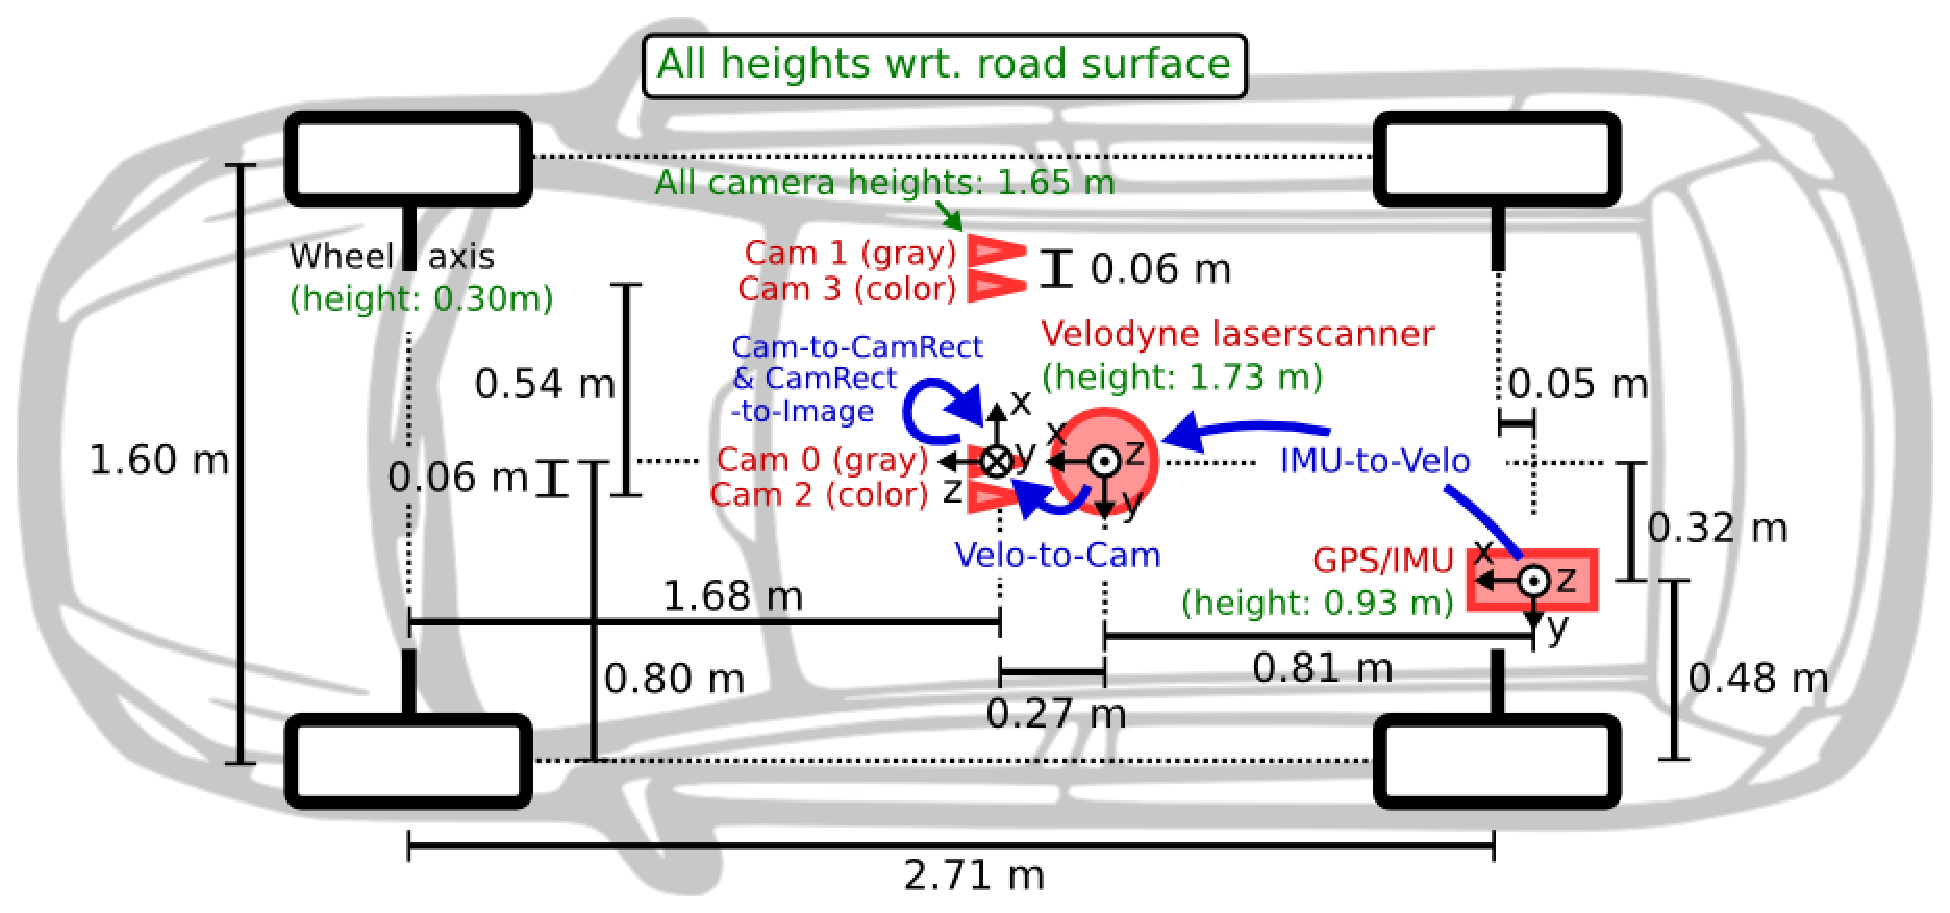
\includegraphics[width=6.0in]{self_driver_top_view}
\caption{A vehicle equipped with four cameras(Cam0\texttildelow Cam3).}
\label{fig:VehicleWithFourCameras}
\end{figure*}
show a typical multi-views system---a vehicle equipped with four cameras to detection objects \cite{Geiger2012::Are}. Some reasons easily cause abnormal images. First, the camera lens were blocked by rain, snow or mosquitoes; Second, losing some information in the process of image signal compression, transmission and decompression. When the autonomous vehicles are running and these unexpected things happened, would lead to traffic accidents. In order to automatically restore the abnormal images on driving, we propose a novel image inpainting method based on multi-views. Our method can be used on other multi-views systems.

\IEEEpubidadjcol
Image inpainting has made tremendous progress in the past nearly two decades. Many methods has been proposed which can be divided into two sets. The first set of approaches relies on texture synthesis techniques, which fills in the hole by extending the textures of the surrounding area \cite{Efros1999::Texture,Drori2003::Fragment,Wilczkowiak2005::Hole,Barnes2009:AToG:PatchMatch:}. What these techniques have in common is the use of patches with similar textures to synthesize the content of the hole region from coarse to fine. Drori et al. \cite{Drori2003::Fragment} and Wilczkowiak et al. \cite{Wilczkowiak2005::Hole} introduced multiple scales and orientations to find better matching patches. Barnes et al. \cite{Barnes2009:AToG:PatchMatch:} used the fast approximate nearest neighbor algorithm to search the match patches. Such methods are good at propagating high-frequency texture details. When part ot the object is missing, using these methods can perfect restore, but it's hard to use these methods to reproduce the small object when the whole object is missing. Fig \ref{fig:methods_compare:patchMatch} show the result using Barnes et al. \cite{Barnes2009:AToG:PatchMatch:} method to restore the defective image (Fig \ref{fig:methods_compare:input}). Compare the result with the target (Fig \ref{fig:methods_compare:target}), 
\begin{figure}[!t]
\centering
\subfloat[]{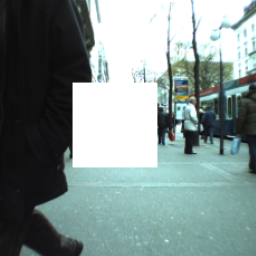
\includegraphics[width=1.0in]{image-introduction-methodsCompare/3-left-image_00000615_0-inputs.png}%
\label{fig:methods_compare:input}}
\hfil
\subfloat[]{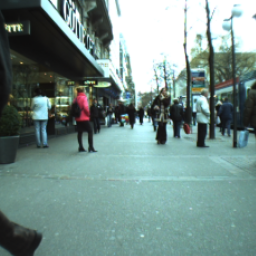
\includegraphics[width=1.0in]{image-introduction-methodsCompare/3-left-image_00000615_0-conditions.png}%
\label{fig:methods_compare:condition}}
\hfil
\subfloat[]{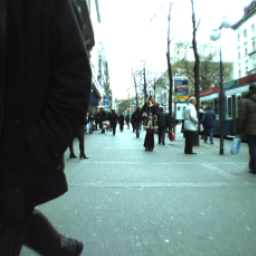
\includegraphics[width=1.0in]{image-introduction-methodsCompare/3-left-image_00000615_0-targets.png}%
\label{fig:methods_compare:target}}
\vfil
\subfloat[]{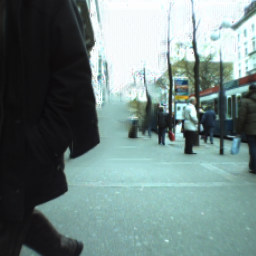
\includegraphics[width=1.0in]{image-introduction-methodsCompare/3-left-image_00000615_0-patchMatch_output.png}%
\label{fig:methods_compare:patchMatch}}
\hfil
\subfloat[]{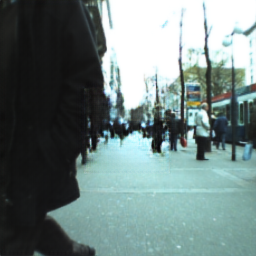
\includegraphics[width=1.0in]{image-introduction-methodsCompare/3-left-image_00000615_0-noMultiViews_outputs.png}%
\label{fig:methods_compare:Image2Image}}
\hfil
\subfloat[]{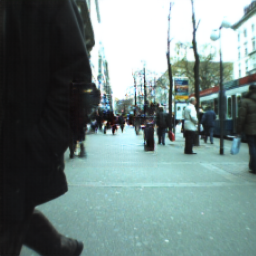
\includegraphics[width=1.0in]{image-introduction-methodsCompare/3-left-image_00000615_0-our_outputs.png}%
\label{fig:methods_compare:ourMethod}}
\caption{Qualitative illustration of the different image inpainting methods. (a) Given an image with a missing region captured by left camera. (b) Given the same scene image captured by right camera. (c) The target of the left image inpainting. (d) PatchMatch method result. (e) Image-to-Image method result. (f) Our method result. }
\label{fig:methods_compare:introduction}
\end{figure}
we can find part of the black coat is restore and some small pedestrians fall in the blank region is not reproduce. The second set of approaches solve this problem in a data-driven way \cite{Hays2007::Scene}, involving a cut-paste formulation using nearest neighbors from a dataset of millions of images. This approach is very effective when it finds an example image with sufficient visual similarity to the query but could fail when the query image is not well represented in the database. A serious problem is that the image restored with this method seems reasonable, but the image content is quite different from the target image. Furthermore, it is struggles to fill arbitrary holes, e.g. objects are partially missing. Additionally, the data-driven way restricts application scenarios.

\IEEEpubidadjcol
With the continuous updating and development of convolutional neural network, various tasks of computer vision have been breakthrough. Image inpainting technology has also been improved. Autoencoders \cite{Hinton2006:s:Reducing,Bengio:Co:Learning} encode image to a low-dimensional "bottleneck", decode it by reconstructing the high-dimensional image from the "bottleneck". The purpose of doing this to obtain the compact feature representation of the scene. Denoising autoencoders \cite{Vincent2008::Extracting} reconstruct the image from corrupted status to learn more robust features. Using  denoising autoencoders to inpaint defective image can get blurred image. 

Pathak et al. \cite{Pathak2016::Context}

This demo file is intended to serve as a ``starter file''
for \textit{IEEE Sensors Letters} papers produced under \LaTeX\ 
\cite{IEEEhowto:kopka} using IEEE\_lsens.cls version 1.0 and later.

I wish you the best of success.

\hfill mds
 
\hfill July 12, 2017

\subsection{Subsection Heading Here}
Subsection text here.

% needed in second column of first page if using \IEEEpubid
%\IEEEpubidadjcol

\subsubsection{Subsubsection Heading Here}
Subsubsection text here.
%\footnote{IEEE Sensors Letters does allow footnotes.}


% An example of a floating figure using the graphicx package.
% Note that \label must occur AFTER (or within) \caption.
% For figures, \caption should occur after the \includegraphics.
% Note that IEEEtran v1.7 and later has special internal code that
% is designed to preserve the operation of \label within \caption
% even when the captionsoff option is in effect. However, because
% of issues like this, it may be the safest practice to put all your
% \label just after \caption rather than within \caption{}.
%
% The IEEE does not put floats in the very first column - or typically
% anywhere on the first/title page for that matter. In addition, IEEE
% Sensors Letters typically puts floats only at the top, even when this
% results in an entire column being occupied by floats. Also, in-text
% middle ("here") positioning is not used. 
%
% Double column floats (i.e., \begin{figure*}, \begin{table*}) should
% not appear on the very first (title) or last pages of IEEE Sensors Letters
% papers.
%
% Also note that IEEE Sensors Letters uses the naming convention of
% fig1.eps, fig2a.pdf, etc., for submitted graphics files.
%
%\begin{figure}[!t]
%\centering
%\includegraphics[width=2.5in]{fig1}
% where an .eps filename suffix will be assumed under latex, 
% and a .pdf suffix will be assumed for pdflatex; or what has been declared
% via \DeclareGraphicsExtensions.
%\caption{Simulation results for the network.}
%\label{fig_sim}
%\end{figure}


% An example of a figure with subfigures using the subfig.sty package.
% (The subfig.sty package must be loaded for this to work.)
% The subfigure \label commands are set within each subfloat command,
% and the \label for the overall figure must come after \caption.
% \hfil is used as a separator to get equal spacing.
% Watch out that the combined width of all the subfigures on a 
% line do not exceed the column width or a line break will occur.
%
%\begin{figure}[!t]
%\centering
%\subfloat[]{\includegraphics[width=1.5in]{fig1a}%
%\label{fig_lossrate_a}}
%\hfil
%\subfloat[]{\includegraphics[width=1.5in]{fig1b}%
%\label{fig_lossrate_b}}
%\caption{Measured and actual loss rates for each stage. (a) $p=0.30$. (b) %$p=0.60$.}
%% or (a), (b) can each carry a complete description:
%%\caption{(a) First description. (b) Second description.}
%\label{fig_lossrate}
%\end{figure}
% Note that IEEE Sensors Letters usually only labels the subfigures
% with (a), (b) and puts all other description within in the main caption.
% With subfig.sty, you still have to invoke the option argument
% (subfig caption) of \subfloat[]{} to get the (a), (b) labels, even if
% the subfig caption/description itself is empty.


% An example of a floating table. Note that, for IEEE style tables, the
% \caption command should come BEFORE the table and, given that table
% captions serve much like titles, are usually capitalized except for words
% such as a, an, and, as, at, but, by, for, in, nor, of, on, or, the, to
% and up, which are usually not capitalized unless they are the first or
% last word of the caption. The \label must come after \caption as always.
%
% Table text will default to \scriptsize as IEEE Sensors Letters normally
% uses this smaller font for tables.
%
% Note that IEEE Sensors Letters uses "open" style tables that do
% not typically use any vertical rules. 
%
% Table example from: S. Banerjee, B. Rana, S. Pauri, S. Chatterjee
% and N. Dey, "HMSIW-Based Miniaturized Sensing Antennas for S- and C-Band
% Applications", IEEE Sensors Letters, February 2017.
%
% IEEEeqnarray version:
%\begin{table}[!t]
%\caption{Comparison of the HMSIW Semi-Circular Antenna With That of a Conventional Semi-Circular Patch Antenna.}
%\label{table_example_antenna}
%\centering
%\begin{IEEEeqnarraybox}[\IEEEeqnarraystrutmode\IEEEeqnarraystrutsizeadd{2pt}{1pt}][b][\columnwidth]{s+t+t}
%\IEEEeqnarraydblrulerowcut\\
%\IEEEeqnarrayseprow[2pt]{}\\
%Antenna parameters&Semi-cicular&HMSIW semi-circular\IEEEeqnarraystrutsizeadd{0pt}{-1pt}\\
%&patch antenna& antenna\IEEEeqnarraystrutsizeadd{-2pt}{-1pt}\\
%\IEEEeqnarrayseprow[2pt]{}\\
%\IEEEeqnarrayrulerow\\
%\IEEEeqnarrayseprow[2pt]{}\\
%Frequency&3.67 GHz&5.22 GHz\\
%Return Loss&-20 dB&-25 dB\\
%Co-polarization Gain&E-plane: 5.8 dBi&E-plane: 6.4 dBi\IEEEeqnarraystrutsizeadd{0pt}{-1pt}\\
%&H-plane: 5.8 dBi&H-plane: 5.3 dBi\IEEEeqnarraystrutsizeadd{-2pt}{0pt}\\
%Directivity&7.2&6.9\\
%Radiation Efficiency&82\%&92\%\\
%Mutual Coupling&-17 dB&-23 dB\\
%\IEEEeqnarrayseprow[4pt]{}\\
%\IEEEeqnarraydblrulerowcut
%\end{IEEEeqnarraybox}
%\end{table}
%
%
% Tabular version, loading the array.sty package is recommended:
%\begin{table}[!t]
%\caption{Comparison of the HMSIW Semi-Circular Antenna With That of a Conventional Semi-Circular Patch Antenna.}
%\label{table_example_antenna_tabular}
%\centering
%% increase table row spacing, adjust as needed
%\renewcommand{\arraystretch}{1.4}
%% if using array.sty, you can tweak the value of \extrarowheight
%% as needed to properly center the text within the cells
%\begin{tabular*}{\columnwidth}{l@{\extracolsep{\fill}}c@{\extracolsep{\fill}}c}
%\hline
%\hline
%Antenna parameters&Semi-cicular&HMSIW semi-circular\rule{0pt}{10pt}\\
%\noalign{\vskip -3pt}&patch antenna& antenna\rule[-5pt]{0pt}{5pt}\\
%\hline
%Frequency&3.67 GHz&5.22 GHz\rule{0pt}{10pt}\\
%Return Loss&-20 dB&-25 dB\\
%Co-polarization Gain&E-plane: 5.8 dBi&E-plane: 6.4 dBi\\
%\noalign{\vskip -3pt}&H-plane: 5.8 dBi&H-plane: 5.3 dBi\\
%Directivity&7.2&6.9\\
%Radiation Efficiency&82\%&92\%\\
%Mutual Coupling&-17 dB&-23 dB\rule[-6pt]{0pt}{6pt}\\
%\hline
%\hline
%\end{tabular*}
%\end{table}



\section{Conclusion}
The conclusion goes here.



% use section* for acknowledgment
\section*{Acknowledgment}
% addcontentsline needed when using bookmark hyperlinking, etc.
\addcontentsline{toc}{section}{Acknowledgment}
% enable scriptsize
\scriptsize
This work was supported by the IEEE. The authors would
like to thank ... Note that the Acknowledgment section of
\textit{IEEE Sensors Letters} is rendered in scriptsize.

% put at least one blank line to end the scriptsize paragraph and
% then revert back to normalsize.
\normalsize


% Last page column equalization
%
% IEEE Sensors Letters does balance the columns on the last page.
% Can use:
% \IEEEtriggeratref{8}
% to trigger a \newpage just before the given reference number to
% balance the columns on the last page. Adjust the reference number
% as needed - this may need to be readjusted if the document is 
% modified later.
% The "triggered" command can be changed if desired:
%\IEEEtriggercmd{\enlargethispage{-5in}}
%
% Alternatively, you can also directly use something like
% \enlargethispage{-7in}
% on the last page instead of breaking at a specific reference number.


% references section
%
% can use a bibliography generated by BibTeX as a .bbl file
% BibTeX documentation can be easily obtained at:
% http://mirror.ctan.org/biblio/bibtex/contrib/doc/
% The IEEEtran BibTeX style support page is at:
% http://www.michaelshell.org/tex/ieeetran/bibtex/
\bibliographystyle{IEEEtran}
% argument is your BibTeX string definitions and bibliography database(s)
\bibliography{/mnt/hgfs/Downloads/refer-frizy/refer-frizy}
%
% Before submitting to IEEE Sensors Letters, manually copy in the
% resultant .bbl file contents in place of the \bibliographystyle and
%\bibliography lines here:
\begin{thebibliography}{1}

\bibitem{IEEEhowto:kopka}
H.~Kopka and P.~W. Daly, \emph{Guide to \LaTeX}, 4th~ed.\hskip 1em plus
  0.5em minus 0.4em\relax Boston, MA: Addison-Wesley, 2004.

\end{thebibliography}



% that's all folks
\end{document}


